\documentclass[12pt]{article}

\setlength\parindent{0pt}
\newcommand{\myt}[1]{\textbf{\underline{#1}}}

\usepackage{mathtools}
\usepackage{amssymb}
\usepackage{tikz,ifthen,amsmath,amssymb,fancyhdr,comment,lastpage}
\usepackage{graphicx}

\title{\vspace{-15ex}Module 7 - Dictionaries for Multi-Dimensional Data\vspace{-1ex}}
\date{July 2nd, 2015}
\author{Graham Cooper}

\begin{document}
	\maketitle
	
	\section*{Ranged Dictionaries}
	\begin{itemize}
		\item insert/delete
		\item range search (look for everything within a range)
	\end{itemize}
	
	\section*{Skip Lists}
	Lists which contain a list on the bottom level of all of the nodes, and have a chance of adding 1 to the height of 1/2 until it fails. We can then check only the lists on each level and snake our way to the correct node looking for boundaries\\
	
	\subsection*{Analysis of Skip Lists}
	If there are n nodes in $S_i$ then it is expected to have $\frac{n}{2}$ at level $S_{i+1}$ number of nodes in a skip list of n items is expected to be:\\
	$$n + \frac{n}{2} + \frac{n}{4} + ... + 1 = n\underset{< 2}{(1 + \frac{1}{2} + ...)} \in \Theta(n)$$
	
	\subsection{Search}
	Number of nodes visited of a list $S_i$ = distance between the two consectuive nodes in $S_{i+1} \in \Theta(n)$ (1 + 1/2 + ...)\\
	Number of levels $\in \Theta(logn)$ is what it is expected to be\\
	
	Search $\in \Theta(logn)$\\
	
	\section{Range Search}
	A=
	\begin{tabular}{|c | c | c | c | c | c | c | c |}
		\hline
		6 & 2 & 3 & 9 & 1 & 8 & 20 & 0 \\ \hline
	\end{tabular}
	
	\begin{itemize}
		\item Array(linked list) - RangeSearch takes $\Theta(n)$
		\item Sorted Array - BS the boundaries - $\Theta(logn + k)$ where k is the number of reported items. However, insert and delete takes $\Theta(n)$
		\item Balanced BST\\
		- Internal Nodes (check)\\
		- External Nodes X\\
		- Boundary Nodes ?\\
	\end{itemize}
	
	\section*{2Dimensional Range-Search}
	\begin{enumerate}
		\item flatten two dimensions (like hashing) (rabge-search becomes hard)
		\item Maintain a dictionary for each dimension (not effective)
		\item Quad trees, kd-trees, Range-trees
	\end{enumerate}
	
	\section*{Quad-Trees}
	
	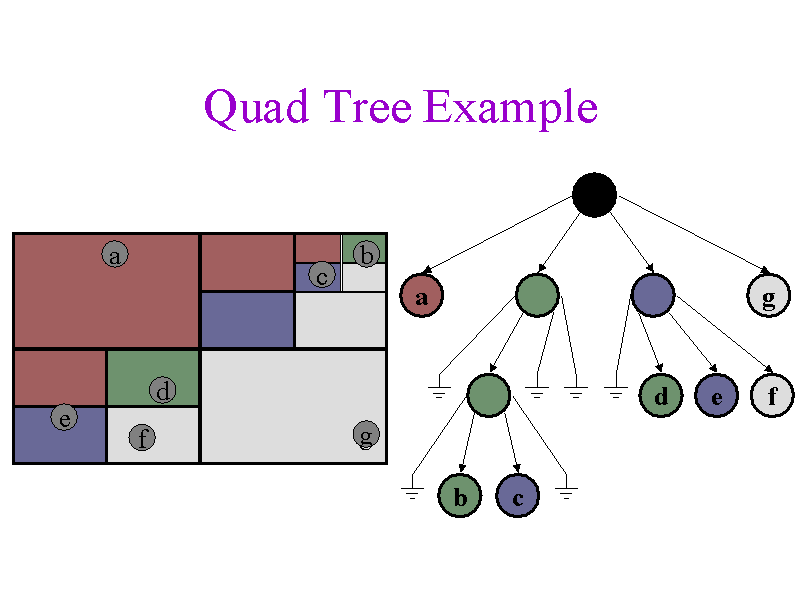
\includegraphics[scale=0.5]{quad-tree.png}\\
	
	Spread factor = $\frac{d_{max}}{d_{min}}$\\
	height of quad tree $\Theta(log(\frac{d_{max}}{d_{min}})$\\
	
	
\end{document}